%% This is an example first chapter.  You should put chapter/appendix that you
%% write into a separate file, and add a line \include{yourfilename} to
%% main.tex, where `yourfilename.tex' is the name of the chapter/appendix file.
%% You can process specific files by typing their names in at the 
%% \files=
%% prompt when you run the file main.tex through LaTeX.
\chapter{Motivación del diseño y desarrollo de XRemoteBot}\label{cha:motivacion}

En este capítulo se relatan los motivos que llevaron a implementar XRemoteBot como
parte de esta tesina, como así también se aclaran algunas decisiones iniciales de
diseño y la desición del lenguaje de programación en el cuál se implementará la mayor
parte del sistema.

% FIXME ¿una intro al cap?

\section{Motivación}\label{sec:motivacion}
Desde el año 2009, en el marco del proyecto ``Programando con robots y
software libre'' de la Facultad de Informática,
se utilizan robots para brindar cursos básicos de programación en Python a alumnos de escuelas
secundarias. Estos robots son simplemente una herramienta didáctica, dado que el foco principal es la enseñanza de las estructuras básicas de Python y no la electrónica relacionada a los mismos.

%FIXME aca no se si no pondría un párrafo de por qué python... fijate en el libro de robots qué pusimos...

%FIXME FIJATE SI PODES HACER QUE LAS FIGURAS SE MUESTREN MAS CERCA DE DONDE LAS MENCIONAS

\begin{figure}
    \centering
    \begin{subfigure}[b]{0.49\textwidth}
        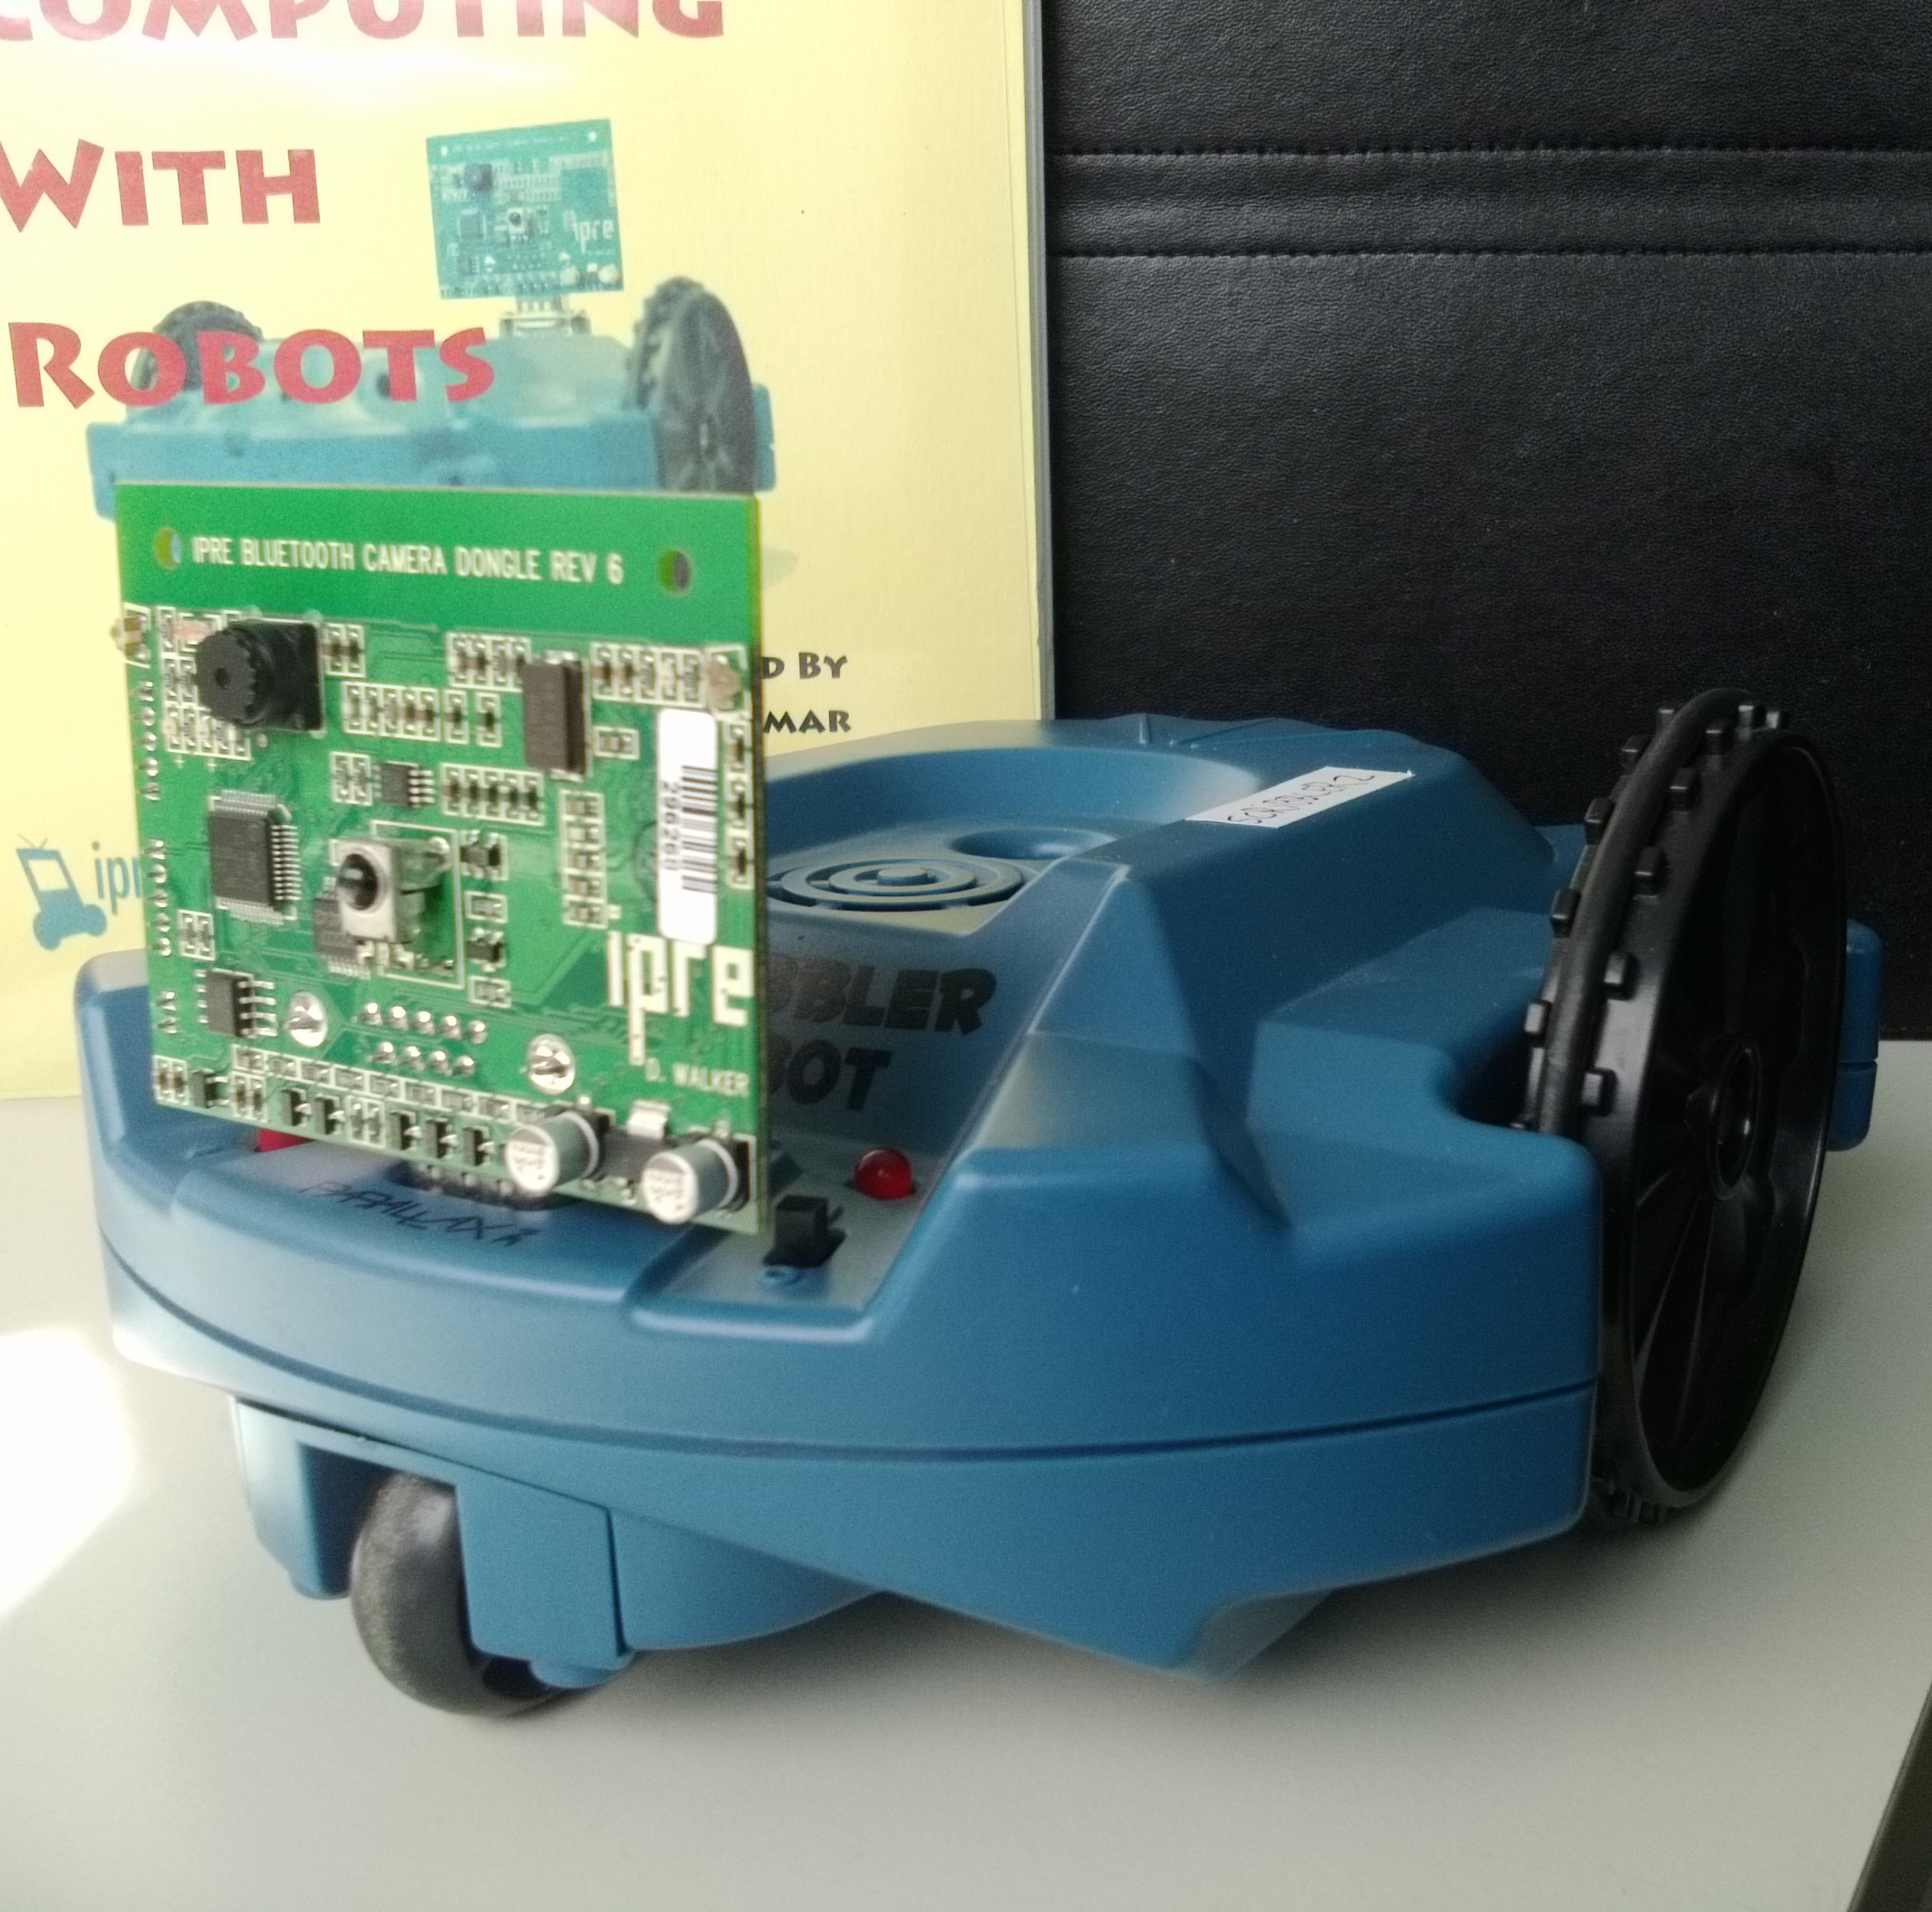
\includegraphics[width=\textwidth]{figures/scribbler}
        \subcaption{Robot Scribbler de Parallax}\label{fig:robots_usados_scribbler}
    \end{subfigure}
    \begin{subfigure}[b]{0.49\textwidth}
        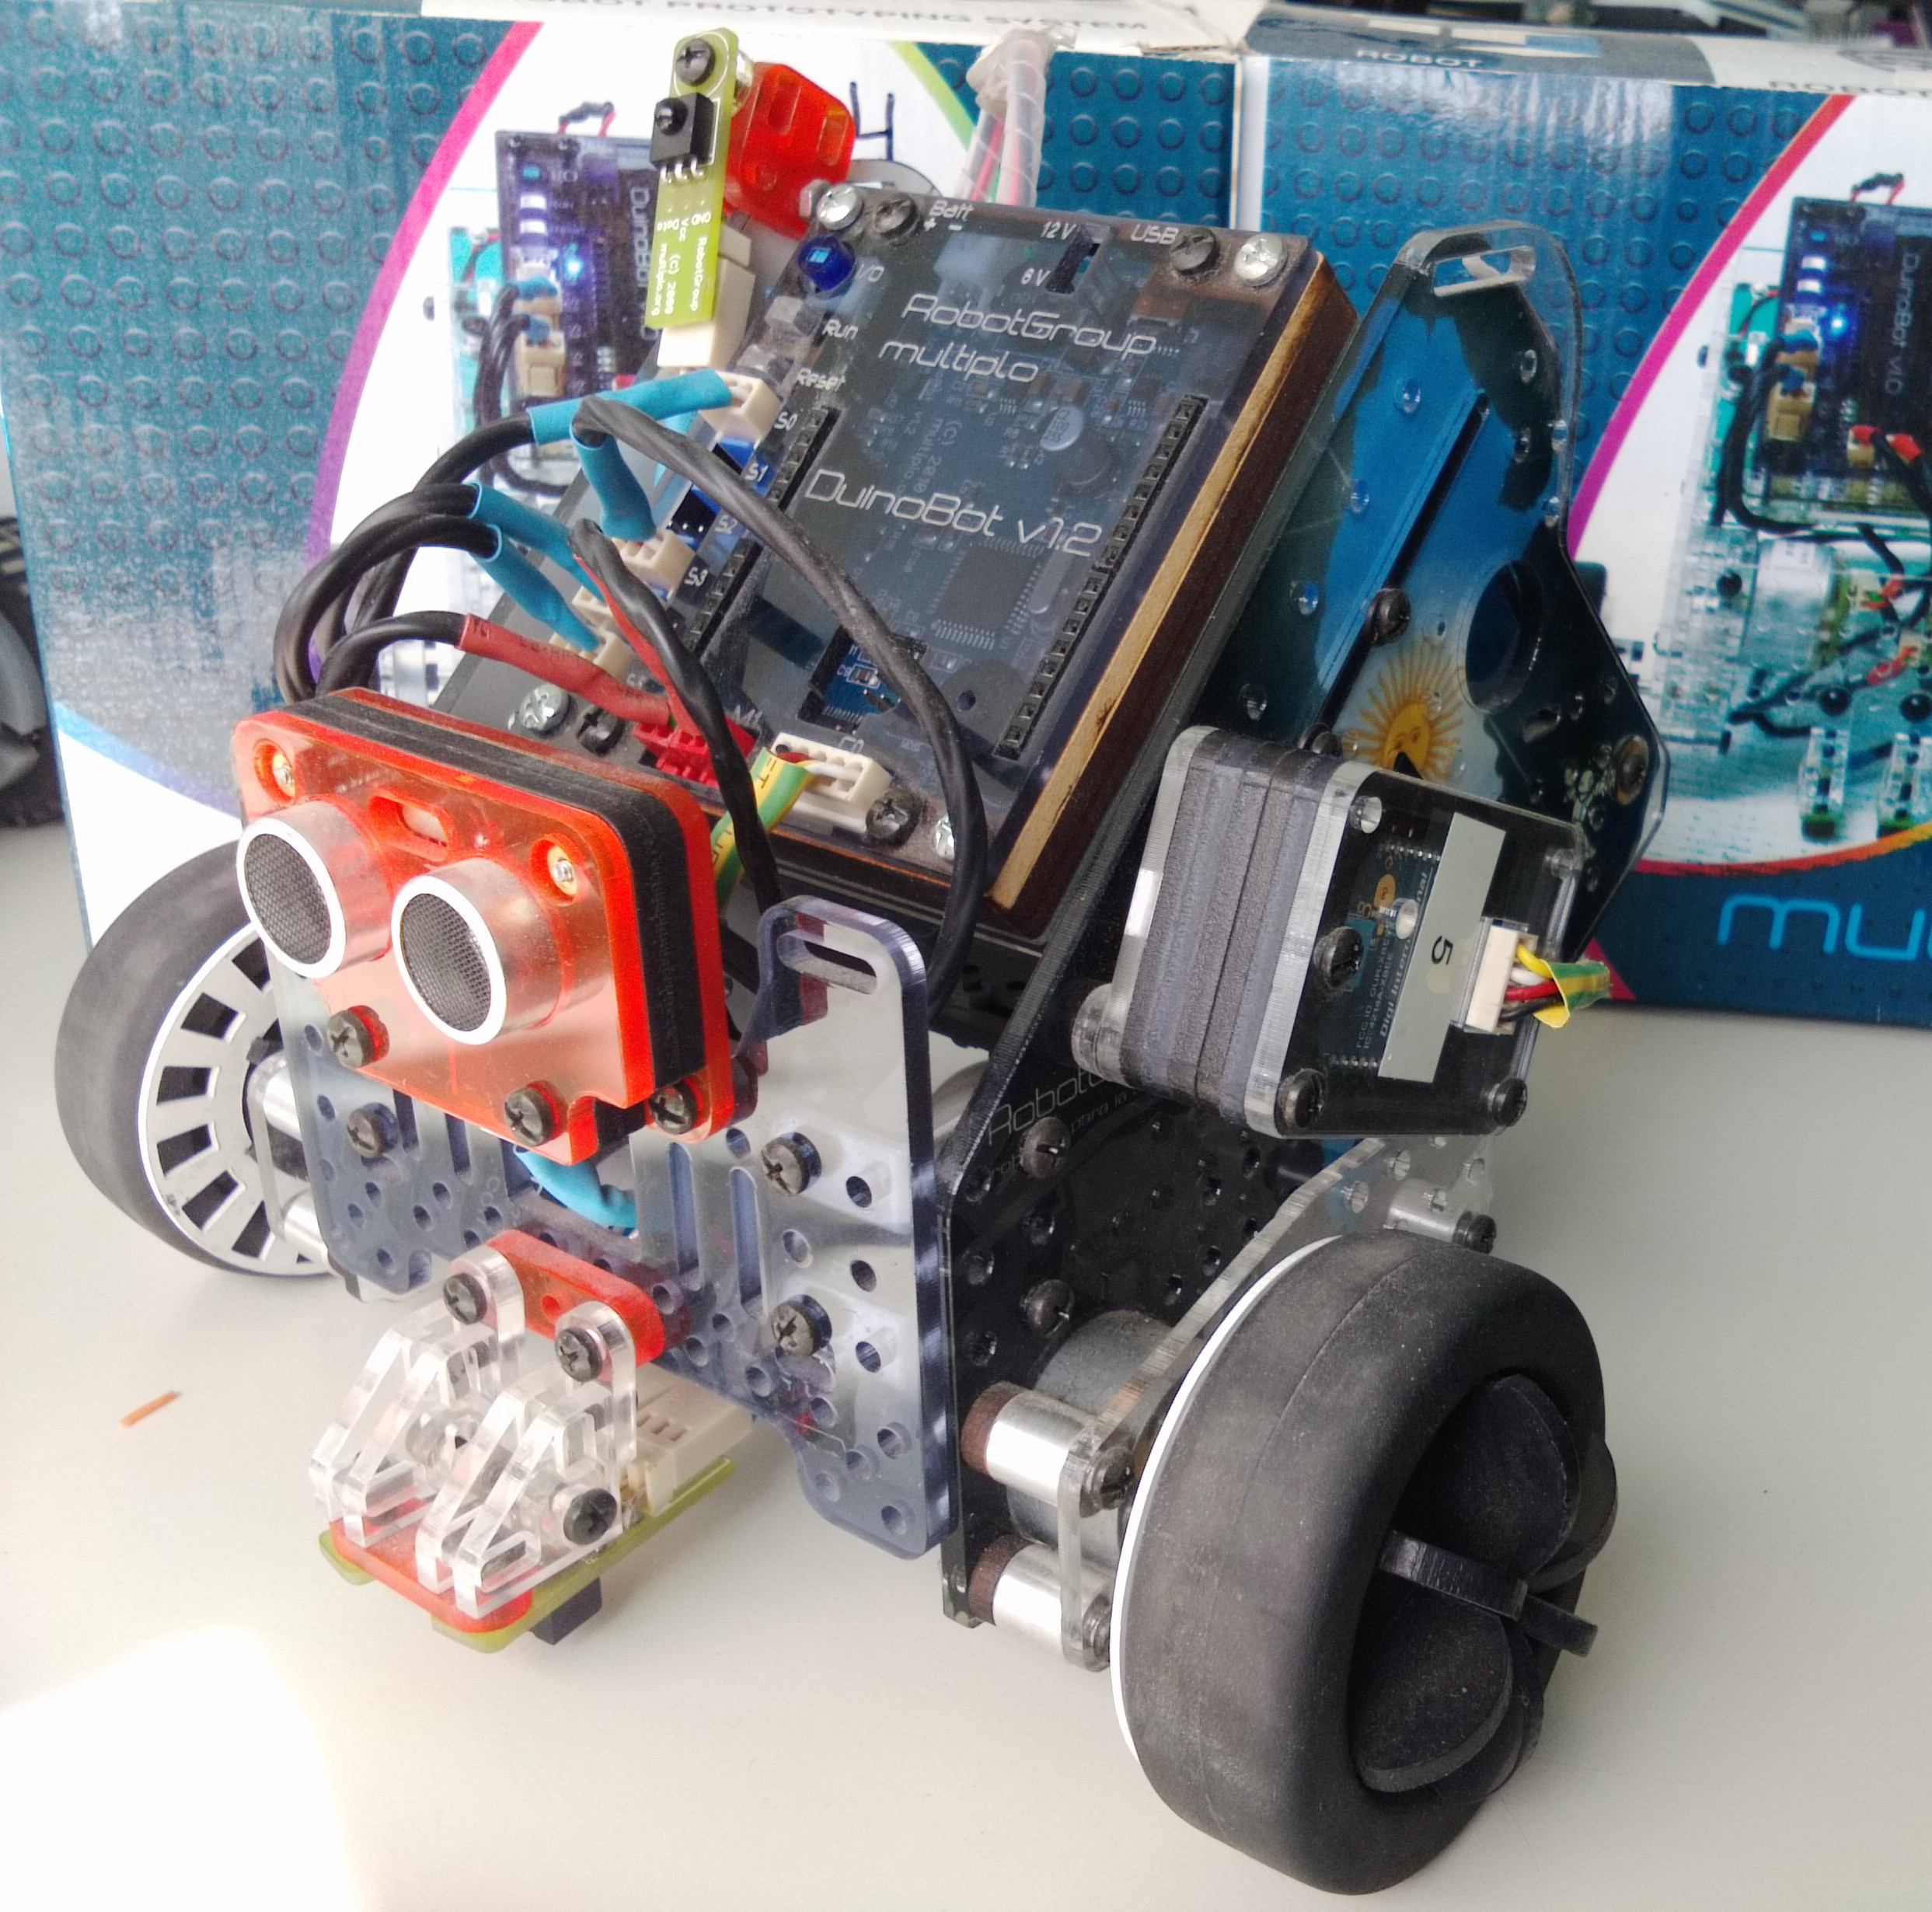
\includegraphics[width=\textwidth]{figures/n6}
        \subcaption{Robot Multiplo N6 de RobotGroup}\label{fig:robots_usados_n6}
    \end{subfigure}
    \caption{Robots usados en el proyecto}\label{fig:robots_usados}
\end{figure}

En un comienzo se utilizaron los robots Scribbler de Parallax, mostrados en la figura~\ref{fig:robots_usados_scribbler}. Estos robots pueden programarse directamente a través de un cable utilizando  el lenguaje
PBASIC, y funcionar de forma autónoma o pueden ser controlados de forma
inalámbrica con Bluetooth. En las experiencias realizadas se los utilizó de la última
forma, dado  que permite controlar el robot usando el lenguaje Python, cuyo intérprete no
es posible ejecutar directamente sobre el microcontrolador del mismo.

Estos robots se importaban desde Estados Unidos en volúmenes bajos, lo que
dificultaba su adquisición tanto por el equipo del proyecto como de posibles
escuelas que quisieran comprarlos, dejando, además al equipo sin ninguna garantía
ante posibles averías. Por estos motivos se buscaron alternativas de fabricación nacional,
que pudieran ser programados en lenguaje Python y tuvieran especificaciones abiertas.
De esta manera, a fines del año 2011, se adquirieron dos robots Multiplo N6 de
fabricación nacional por
la empresa RobotGroup, mostrados en la figura~\ref{fig:robots_usados_n6},
tanto el software necesario para controlar estos robots como sus
especificaciones distribuyen bajo una licencia
abierta~\footnote{\url{https://www.kickstarter.com/projects/1689254125/multiplo-create-your-own-robot/description}}.

Los robots Multiplo están basados en
Arduino\footnote{\url{http://www.arduino.cc/}}
por lo que pueden ser programados
usando el IDE Arduino en C++, además RobotGroup ofrece el entorno de programación
MiniBloq que permite programar el robot de forma gráfica usando bloques.
Dado que estas modalidades no se adecuaban a las propuestas del proyecto
se pidió a la empresa una versión modificada del robot para controlarlo de forma
inalámbrica\footnote{Ya que no es posible ejecutar un intérprete cPython en una
placa de esas características.} y se
desarrolló
una biblioteca Python que permite la programación del robot en dicho lenguaje. Este
desarrollo fue realizado por un equipo de trabajo integrado por miembros del
laboratorio LINTI y miembros de la empresa RobotGroup, y actualmente está
siendo mantenido por el LINTI~\citep{diaz_aprendiendo_2012}.
% FIXME: la cita de estos parrafos está más completa en el paper que cité
% que en ~\citep{lanfranco_2012}. Pongo la ref para cuando se hable de Firmata

La placa
controladora del Multiplo N6 se denomina DuinoBot y no debe confundirse con la biblioteca
Python del mismo nombre que se desarrolló en conjunto con la empresa RobotGroup
para controlar estos robots. De aquí en adelante se denominará DuinoBot a la
biblioteca y placa controladora al componente de hardware que contiene el
microcontrolador a menos que se especifique lo contrario.

En el año 2012, a través de una cooperación con la Fundación YPF que brindó
un subsidio y bajo el auspicio de la Dirección de Escuelas Técnicas de la
Provincia de Buenos Aires se dictaron cursos en 10 escuelas técnicas de la
provincia. La fundación YPF brindó a cada una de estas escuelas, entre otras
cosas, 20 robots Multiplo N6 que quedaron en cada escuela. En estos cursos
se capacitaron más de 140 docentes y 40 alumnos avanzados, en programación
en el lenguaje Python utilizando
estos dispositivos~\citep{diaz_aprendiendo_2012} como herramienta didáctica.

Esta experiencia consolidó el uso de
los robots Multiplo N6 para los cursos dictados en el marco del proyecto
``Programando con robots y software libre'',  donde este nuevo modelo de  robot desplazó
a los Scribblers, tanto por su confiabilidad y la facilidad de adquisición de los mismos.



\section{Los robots}
Como se mencionó anteriormente se utilizaron a lo largo del proyecto dos
modelos de robots distintos: el Scribbler y el Multiplo N6. Esta sección provee una
breve reseña de sus características técnicas.

\subsection{Robot Scribbler de Parallax}
Los robots Scribbler (versión 1) cuentan con un microcontrolador
\textit{PIC16F57}\footnote{Esta información se obtuvo con una inspección
visual de uno de estos robots.}
que viene programado con un intérprete de Basic. El producto
completo es denominado por Parallax
``Basic Stamp 2''\footnote{\url{http://www.andybrain.com/extras/scribbler-robot-review.htm}}.
Para su locomoción este robot cuenta con dos ruedas conectadas a través de
cajas
reductoras
% FIXME por ahí mejo no ponerlo y listo
% \footnote{\url{http://es.wikipedia.org/wiki/Reductores_de_velocidad}}
a sus respectivos motores de DC (corriente continua)  y una tercer rueda no conectada a ningún
motor que sirve como tercer punto de apoyo para el cuerpo del robot.

La alimentación eléctrica del robot es provista por 6 pilas AA.

En cuanto a los sensores, este robot está equipado con:
\begin{itemize}
    \item Dos emisores infrarrojos a los lados de su parte frontal y un
        sensor infrarrojo entre ellos que permite sensar (de acuerdo a si se
        refleja el haz de luz infrarroja de alguno de los laterales) si
        hay algún obstáculo a la derecha o a la izquierda del robot.
    \item Tres fotorresistores ubicados dentro de 3 cavidades al frente del
        robot que permiten sensar la presencia de fuentes de luz e
        identificar (si la luz no es muy difusa) si las mismas se encuentran
        directamente enfrente, a la izquierda o a la derecha del robot.
    \item Dos sensores de línea que consisten cada uno de un emisor
        y un sensor infrarrojo (IR). Los mismos detectan cambios de contraste
        en el piso de acuerdo a la cantidad de luz IR reflejada y generalmente
        se utilizan para que el robot siga un camino demarcado por una línea
        de un color sobre una superficie de un color contrastante.
\end{itemize}

Si bien las anteriores son las características generales de estos robots, usándolos
de esta manera es necesario programarlos a través de un cable serial usando el
lenguaje PBASIC basado en BASIC. Para las actividades planteadas en el marco del
proyecto \proyecto{}, se utilizó  una versión
que agrega un dispositivo extra: el IPRE Fluke. Este dispositivo se conecta al puerto
serial del robot y provee la capacidad de comandarlo de forma inalámbrica
usando Bluetooth.  Conectar el
IPRE Fluke invierte el sentido de giro de las ruedas, por lo que el frente
del robot pasa a ser el lugar donde se conecta el IPRE Fluke. De aquí
en adelante cuando se mencione la parte delantera del Scribbler, será la
parte donde se encuentra conectado el IPRE Fluke y la parte trasera será la
opuesta.

El IPRE Fluke es comandado por con un microcontrolador
\textit{LPC2106F}\footnote{Información obtenida con una inspección visual
de la placa.}
basado en la arquitectura
\textit{ARM7}\footnote{\url{http://pdf1.alldatasheet.com/datasheet-pdf/view/83950/PHILIPS/LPC2106FHN48.html}}
. Posee un módulo de comunicaciones
Bluetooth que utiliza como medio de comunicación con la computadora
controlante y
provee una cámara de baja resolución con la que se pueden tomar fotografías
que luego serán transmitidas por bluetooth. Además agrega
un sensor infrarrojo que permite detectar la presencia de obstáculos
a la izquierda, al centro o a la derecha (está compuesto de 3 emisores
y un
receptor)\footnote{\url{http://wiki.roboteducation.org/Myro_Hardware}}.
Con esta adición el robot queda equipado ahora con sensores
en la parte frontal y en la parte trasera, pero más importante aún
el módulo Bluetooth permite controlarlo de forma inalámbrica siempre
que se grabe un firmware especial en la placa IPRE Fluke. Esto es lo que permite
que estos robots puedan ser programados con Python unsando una biblioteca denominada
\textit{Myro}, que será descripta más adelante en este informe.

\subsection{Multiplo N6}
El robot Multiplo N6, fabricado por la empresa RobotGroup, cuenta con un
microcontrolador Atmel
\textit{AVR ATMega32U4}\footnote{\url{http://www.robotgroup.com.ar/index.php/productos/131-robot-n6\#especificaciones}}
con el bootloader de Arduino
precargado. Para su locomoción cuenta con dos ruedas conectadas a través
de reductores de velocidad a sus correspondientes motores DC y una tercer
rueda no conectada a ningún motor que sirve como tercer punto de apoyo.
La alimentación eléctrica de estos robots está dada por tres pilas AA
en serie (o bien dos packs de tres pilas cada uno en paralelo).

En cuanto a los sensores el Multiplo N6 está equipado con:
\begin{itemize}
    \item Un sensor ultrasónico para detectar obstáculos al frente del
        robot.
    \item Un sensor infrarrojo que puede ser utilizado en conjunto con
        un control remoto universal para enviar comandos al robot
        (siempre que se programe este comportamiento previamente).
    \item Dos sensores detectores de línea, compuestos de un emisor y
        un receptor infrarrojo cada uno.
    \item Opcionalmente estos sensores pueden desatornillarse y ensamblarse
        para funcionar como encoders de las ruedas, de esta manera pudiendo
        calcular la velocidad de giro de las ruedas (pero este uso
        no es recomendable si se controla el robot de forma remota
        ya que la latencia de las comunicaciones puede hacer que se pierdan
        datos haciendo que el cálculo de la velocidad se impreciso).
\end{itemize}

En esta configuración estos robots son programables usando el entorno de
Arduino y desde MiniBloq, pero dado que el objetivo del proyecto es la enseñanza de
programación en el lenguaje Python se encargó a la empresa una versión
modificada del Multiplo N6 que permitiera controlarlo de forma inalámbrica,
de manera tal que una computadora con un intérprete de Python instalado
pudiera enviar instrucciones y recibir los valores de los sensores
del robot tal y como hace la biblioteca Myro con los robots Scribbler.
Esta
modificación consistió en la adición de un módulo de comunicación inalámbrica
XBee que permite enviar y recibir datos del robot a través del protocolo
ZigBee\footnote{\url{http://www.digi.com/xbee/}}, la modificación de
un firmware basado una implementación existente para Arduino del protocolo
de control \texttt{Firmata}\footnote{\url{http://firmata.org/}} y
el módulo Python \texttt{Duinobot} para controlar a los robots usando
este protocolo, el
cuál fue adaptado por los miembros del proyecto \proyecto{}
para soportar nuevas funcionalidades y proveer una
API similar a la de la biblioteca
\texttt{Myro}\citep{lanfranco_2012}.

Básicamente los Multiplo N6 utilizados en el proyecto \proyecto{} vienen
con este firmware basado en Firmata (pero modificado a fin de soportar
las características propias del robot) que recibe instrucciones desde
un un puerto serie conectado a una placa XBee y envía las respuestas
al mismo utilizando una variación del protocolo Firmata. Desde el lado
de la computadora controlante, el módulo Duinobot provee una interfaz
de alto nivel para los alumnos donde cada instrucción para el robot
programada
en Python se convierte a una secuencia de bytes del protocolo Firmata
y se envía al robot a través de una placa XBee conectada por USB a la
computadora y cada respuesta del robot se almacena para ser utilizada
como valor de respuesta en los métodos asociados con los sensores.


\section{Características comunes}
Aunque se han utilizado a la fecha estos dos modelos distintos de robots,
en esencia, las características principales de ambos modelos son las mismas
y coinciden con las de otros robots usados en la Argentina para enseñar a
programar. En general, todos ellos incluyen:
\begin{itemize}
    \item Un medio de locomoción  con 2 motores continuos que mueven cada
        uno una de las ruedas laterales.
    \item Sensores que permiten detectar obstáculos.
    \item Sensores que permiten detectar líneas.
    \item Operación inalámbrica.
\end{itemize}

Cabe destacar sobre este último ítem que otros robots no requieren
cables para operar ya que son programados
a través de algún lenguaje compilado como C, Assembler
o Basic, se les transfiere el programa a través de un
cable (usualmente USB o Serial)
y este programa se graba en la memoria del microcontrolador permitiendo
que el robot posteriormente ejecute el programa de forma autónoma.
Pero los robots usados en el proyecto antes mencionado no requieren
cables ya que son controlados a través de señales
inalámbricas, lo que permite controlarlos en tiempo real y utilizando
un intérprete Python estándar (cPython) instalado en el dispositivo
controlante.

Dado el costo y fragilidad de los robots habitualmente los alumnos interactúan
con los mismos solamente en el aula, ya sea en su escuela si la misma pudo
adquirir los robots, o en las instalaciones de la  Facultad de Informática si el alumno
realiza alguna pasantía o práctica en la misma. Esto tiene varias connotaciones:
\begin{itemize}
    \item El alumno, al estar en una situación formal en la escuela
        compartiendo el robot (recurso limitado) con otros
        alumnos, posiblemente no tenga el tiempo o el ambiente más apropiado
        para experimentar de forma lúdica con el mismo.
    \item La tarea para casa solamente es realizable a través de un simulador
        que puede ser lo suficientemente completo y fiel como para aprender
        a programar, pero resulta menos estimulante y realista que manipular
        un robot real.
    \item Alumnos de escuelas que no tienen los recursos necesarios para
        adquirir el equipamiento o de escuelas alejadas de La Plata que
        no tienen la posibilidad de acercarse a nuestra
        Facultad no pueden interactuar con robots reales
        (a lo sumo podrán usar un simulador).
\end{itemize}

Por otro lado las placas
XBee que permiten conectarse con los robots Multiplo N6
son relativamente costosos, el esquema normal de conexionado entre dispositivos
controladores y robots descripto en el capítulo~\ref{cha:arquitectura} requiere
2 placas XBee por robot, una conectada directamente al robot y la otra
conectada por USB al dispositivo controlante. En consecuencia:
\begin{itemize}
    \item El dispositivo controlante debe tener un puerto USB y los drivers
        necesarios para detectar la interfaz serial con el XBee, esto deja
        fuera de juego celulares y tablets.
    \item El costo de operar cada robot en este esquema es sensiblemente
        superior al costo que tendría si varios alumnos pudieran
        controlar varios robots usando un solo dispositivo XBee compartido
        entre varios dispositivos controlantes.
\end{itemize}

Tomando estos dos grupos de problemáticas se propone implementar una solución
que permita
superarlos de forma simultánea, esta solución permite controlar los
robots a través de una red, como puede ser Internet, permitiendo a los alumnos
conectarse a los robots desde sus hogares y a las instituciones a compartir
el uso de sus robots. Por otro lado también es posible configurar el servidor
para su uso en el aula deshabilitando funcionalidades innecesarias en un ámbito
local como ser la necesidad de autenticar a los usuarios para utilizar los
robots, este modo de operación fue pensado para que múltiples alumnos puedan
acceder a múltiples robots contando con un solo adaptador USB a XBee, esto
reduciría sensiblemente el costo de cada robot por alumno ya que de otra
manera por cada robot deberían usarse 2 dispositivos XBee (uno en el robot
y otro en la computadora del alumno) reduciéndose con este modo de operación
a un XBee por robot más un único adaptador USB a XBee conectado al servidor.

Como consecuencia de estos requerimientos quedaba claro que el servidor
debía tener una interfaz web y proveer acceso concurrente con relativa
baja latencia para permitir a múltiples alumnos acceder a múltiples robots
al mismo tiempo.
Tener un servidor web basado en protocolos estándar hizo
que el requerimiento de que el cliente estuviera escrito en Python fuera
artificial dado que sería posible implementar clientes en cualquier lenguaje
que soporte estos protocolos. Esto dio lugar a la posibilidad de
implementar otros clientes que permitieran usar los robots en cursos
de programación de distintos lenguajes sin reimplementar el protocolo
de bajo nivel lo que hace en opinión del autor más sencilla la creación
de nuevos clientes en distintos lenguajes.
En especial la elección de protocolos y tecnologías usadas
y la falta de necesidad de acceder directamente al hardware a través de USB,
habilita la implementación de un cliente Javascript que se ejecute en el
navegador Web de los usuarios. Esta implementación, junto con las desarrolladas
en Ruby y Python, se describen en el capítulo~\ref{cha:clientes}.

El nivel de abstracción que puede proveer esta API hace que sea
una consecuencia natural de este diseño pensar
pensar en la posibilidad de manejar distintos tipos de robots
que tengan algunas características mínimas en común con los robots ya
descriptos utilizando la misma interfaz de programación, por lo que
teniendo ciertos cuidados en la implementación del protocolo y el
servidor se puede lograr que ambos sean fácilmente extensibles para
agregar soporte para nuevos robots.

En cuanto al lenguaje de programación utilizado en el desarrollo del servidor,
dado que las bibliotecas utilizadas para controlar los robots Multiplo N6 y
Scribbler se encuentran desarrolladas en Python y dada la experiencia del autor
tanto en el uso de estas bibliotecas como en el uso del lenguaje Python en general
éste es el lenguaje elegido para el desarrollo del servidor, en particular la
versión 2.7 de Python ya que utilizar la versión 3 requeriría extensivas
modificaciones a estas bibliotecas y otras relacionadas.
